\documentclass[border=5pt]{standalone}
\usepackage{tikz}
\usetikzlibrary{calc, angles, quotes}

\begin{document}

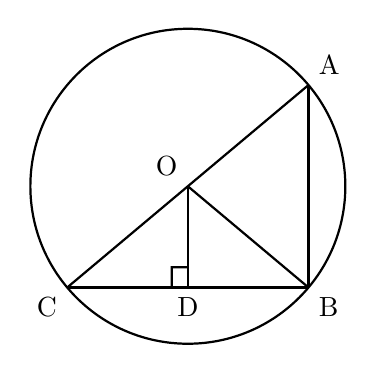
\begin{tikzpicture}[scale=1, thick]

    % 1. Define the Center O and draw the circle
    \coordinate (O) at (0,0);
    \draw (O) circle (2cm);

    % 2. Define Diameter AC (Collinear through center)
    \coordinate (A) at (40:2);
    \coordinate (C) at (220:2);

    % 3. Define Point B on the circle
    \coordinate (B) at (-40:2);

    % 4. Draw all visible lines
    \draw (A) -- (C);       % Diameter AC
    \draw (A) -- (B);       % Segment AB
    \draw (C) -- (B);       % Segment CB
    \draw (O) -- (B);       % Segment OB

    % 5. Define Point D as the exact midpoint of CB
    \coordinate (D) at ($(C)!0.5!(B)$);
    \draw (O) -- (D);       % Perpendicular OD

    % 6. Draw the Right Angle Symbol at D (on the left side toward C)
    % This uses the calc library to align perfectly with the slope of CB
    \draw ($(D)!0.2!(O)$) --
          ($($(D)!0.2!(O)$)!0.2!90:(O)$) --
          ($(D)!0.16!90:(O)$);

    % 7. Label all points exactly as shown in the image
    \node[above right] at (A) {A};
    \node[below right] at (B) {B};
    \node[below left] at (C) {C};
    \node[above left] at (O) {O};
    \node[below] at (D) {D};

\end{tikzpicture}

\end{document}
